\documentclass[conference]{IEEEtran}
\IEEEoverridecommandlockouts
% Template version as of 6/27/2024

\usepackage{cite}
\usepackage{amsmath,amssymb,amsfonts}
\usepackage{graphicx}
\usepackage{textcomp}
\usepackage{xcolor}
\usepackage[colorlinks=true,linkcolor=red,citecolor=green,urlcolor=blue]{hyperref}
\usepackage{orcidlink}
\def\BibTeX{{\rm B\kern-.05em{\sc i\kern-.025em b}\kern-.08em
    T\kern-.1667em\lower.7ex\hbox{E}\kern-.125emX}}
\hypersetup{
  pdftitle={Exploiting More Than Symmetry in Variational Quantum Machine Learning},
  pdfauthor={Markus Baumann and Claudia Linnhoff-Popien},
  pdfsubject={Variational quantum learning and equivariant ansatz design},
  pdfkeywords={quantum machine learning, equivariance, symmetry, inductive bias, variational quantum circuits, parameter sharing, generalization}
}
\newcommand{\orcid}[1]{\,\orcidlink{#1}}

\begin{document}

\title{Exploiting More Than Symmetry in Variational Quantum Machine Learning\thanks{Corresponding author: \href{mailto:markus.baumann@campus.lmu.de}{markus.baumann@campus.lmu.de}}}

\author{%
\IEEEauthorblockN{Markus Baumann\textsuperscript{*}\orcid{0009-0007-3575-1006} and Claudia Linnhoff-Popien\textsuperscript{*}\orcid{0000-0001-6284-9286}}
\IEEEauthorblockA{\textit{\textsuperscript{*}QAR-Lab, Department of Computer Science, LMU Munich, Munich, Germany}}
}

\maketitle

\begin{abstract}
Symmetry is one of the most powerful priors we can give a learning model: it marks the variations in the input that should leave the answer unchanged, so the model need not learn them from data. The prior is especially valuable in quantum machine learning, where circuits are small and easily overwhelmed, and recent work shows that building a known symmetry into a variational quantum circuit improves generalization. We ask what comes next: once a model is symmetric, is the only choice how much symmetry to impose, or also which symmetry-respecting interactions it may learn? Treating symmetry as a design space, we relax it toward smaller subgroups and find that weaker constraints recover almost all of the benefit, then keep the symmetry but enrich it with trainable interactions acting directly on the patterns that determine the label. This second move lifts performance well beyond the original symmetric circuit, and a control that scrambles the parameter sharing at matched size confirms the gain comes from the task's geometry, not a smaller model. We demonstrate this on Tic-Tac-Toe board classification, chosen because every relevant symmetry, label, and decisive pattern is known exactly, so the effect can be isolated rather than inferred. A known symmetry is not merely a way to tie parameters; it is a language for deciding which interactions a model may learn, and so it is not the end of architecture design but its beginning.

\end{abstract}

\begin{IEEEkeywords}
quantum machine learning, equivariance, symmetry, inductive bias, variational quantum circuits, parameter sharing, generalization
\end{IEEEkeywords}

\section{Introduction}
\label{sec:introduction}
A central challenge in variational quantum machine learning is not merely to
build expressive quantum circuits, but to build the right expressive circuits.
Layered parameterized circuits with data re-uploading
~\cite{benedetti2019parameterized,perezsalinas2020data} can be highly flexible,
but flexibility alone is not a design principle. Without architectural
guidance, a model may spend parameters and data on distinctions irrelevant to
the task, while failing to allocate capacity to the structures that determine
the label. The practical question is therefore not only how much expressivity a
quantum model has, but where this expressivity is placed.

Symmetry is one of the few sources of prior knowledge that can be stated
exactly. Consider a target map \(y:\mathcal X \to \mathcal Y\) and a group
\(S\) acting on the input space through transformations
\(V_s:\mathcal X \to \mathcal X\). The task is invariant under \(S\) if
\[
    y(V_s[x]) = y(x)
    \qquad \text{for all } x \in \mathcal X,\; s \in S .
\]
In words, a symmetry specifies transformations of the input that must not
change the correct prediction. A translated image still depicts the same
object, a permuted graph still represents the same graph, and a rotated
Tic-Tac-Toe board still has the same winner. A model that respects this
structure by construction need not rediscover it from data.

This observation is central to geometric deep learning: classical
architectures such as convolutional neural networks organize trainable degrees
of freedom around task symmetries~\cite{cohen2016group}. In quantum machine
learning, geometric quantum machine learning represents known transformations
on the Hilbert space and constrains circuits accordingly
~\cite{larocca2022group,nguyen2024theory}. Related work has developed
group-invariant models, equivariant quantum neural networks,
permutation-equivariant architectures, graph-equivariant circuits, and
symmetry-informed variational ansatze
~\cite{larocca2022group,nguyen2024theory,skolik2023equivariant,sauvage2024building}.

\begin{figure*}[t]
\centering
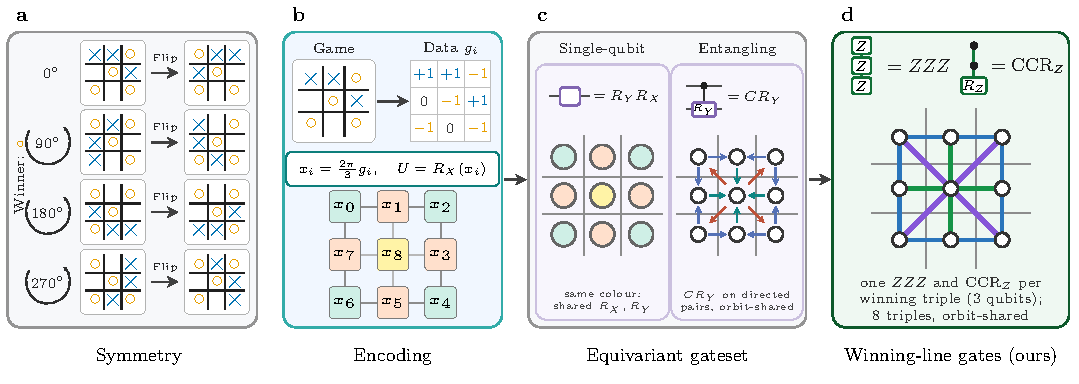
\includegraphics[width=0.98\textwidth]{fig1_4panel_standalone}
\caption{\normalsize From task symmetry to a task-aligned equivariant circuit.
(a) Tic-Tac-Toe labels are invariant under the $D_4$ rotations and reflections of the board.
(b) Board entries $g_i\in\{-1,0,+1\}$ are encoded as $R_X(x_i)$ rotations with $x_i=\frac{2\pi}{3}g_i$; the chosen indexing exposes the corner, side, and center orbits.
(c) The Meyer et al.~\cite{meyer2023symmetry} edge ansatz uses orbit-shared $R_YR_X$ rotations and directed $CR_Y$ entanglers on neighbouring and center-connected fields.
(d) Our extension adds orbit-shared $ZZZ$ and symmetric $CCR_Z$ gates on the eight winning triples, directly matching the label-relevant motifs while preserving equivariance.
Panel layout adapted from Meyer et al.~\cite{meyer2023symmetry}.}
\label{fig:protocol}
\end{figure*}

Meyer et al.~\cite{meyer2023symmetry} gave a concrete blueprint for this
program. If a data embedding \(U(x)\) satisfies
\[
    U(V_s[x]) = U_s U(x) U_s^\dagger ,
\]
then the data symmetry is represented by a unitary action \(U_s\). Trainable
blocks that commute with this representation, together with compatible state
preparation and readout, yield a model whose prediction is invariant by
architecture rather than by optimization.

However, symmetry alone does not specify an ansatz. It tells us which inputs
should be identified, which parameters may be shared, and which observables
should be aggregated, but not where trainable interactions should live. Two
circuits can respect the same group action and still match the task very
differently. We therefore treat symmetry not as a switch, but as a constrained
design space in which one must still choose the sharing strength and the motifs
on which trainable quantum interactions are placed.

Tic-Tac-Toe is a clean laboratory for this question. The task is finite,
exactly enumerable, and structurally transparent: each board has nine fields
and the label is determined by explicit three-cell winning lines. The relevant
symmetry is the dihedral group \(D_4\), containing the eight rotations and
reflections of the square. Acting on a \(3\times3\) board, \(D_4\) permutes the
nine fields while preserving the corner, side, and center orbits. Since these
transformations do not change whether crosses win, circles win, or the game is
a draw, the classification task is \(D_4\)-invariant.

Each board value \(g_i\in\{-1,0,+1\}\) is encoded on one qubit through a
Pauli-\(X\) rotation with angle \(x_i=2\pi g_i/3\). Under a board symmetry, the
encoded qubits are permuted like the board fields, so equivariance can be
imposed by sharing parameters across symmetry orbits of gates.

We separate two design choices that are usually entangled. The first is how
much symmetry to impose: full \(D_4\)-equivariance is natural, but smaller
subgroups may preserve most of the useful bias while leaving the circuit more
flexible. The second is where trainable interactions are placed. The
canonical \(D_4\)-equivariant Tic-Tac-Toe ansatz of Meyer et al. uses
orbit-shared single-qubit rotations and directed controlled rotations on
neighboring or center-connected fields~\cite{meyer2023symmetry}. This respects
the board symmetry, but the label is defined by complete rows, columns, and
diagonals. We therefore add task-aligned, orbit-shared \(ZZZ\) and symmetric
controlled-controlled-\(R_Z\) interactions on these winning triples.

Our numerical results support this design-oriented view. Enforcing board
symmetry improves generalization over an unshared edge ansatz, and suitable
subgroups recover much of the performance of full \(D_4\)-equivariance. The
largest improvement, however, comes from adding winning-line interactions to
the equivariant circuit. Thus, symmetry is not merely a constraint that makes a
model smaller. It is a language for organizing circuit design, but the
effectiveness of the model still depends on placing trainable degrees of
freedom where the structure of the task actually lives.


\begin{figure*}[!t]
\centering
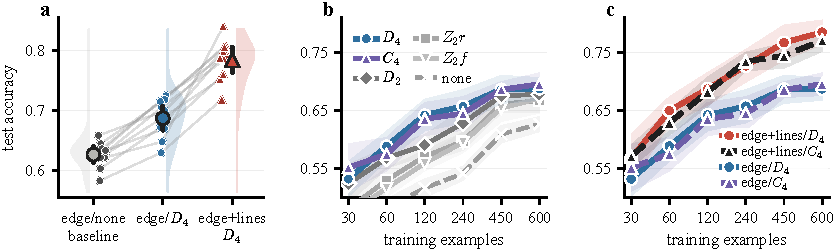
\includegraphics[width=.94\textwidth]{gfx/fig2_main_evidence}
\caption{Main empirical evidence. (a) Full $D_4$ equivariance improves the original edge ansatz over no sharing. (b) The subgroup sweep across training sizes shows that $C_4$ tracks $D_4$ closely. (c) Adding winning-line interactions to the equivariant edge ansatz improves test accuracy while preserving the imposed symmetry.}
\label{fig:main}
\end{figure*}

\section{Protocol}
\label{sec:protocol}
Each legal, reachable board is a list of nine values $g_i\in\{-1,0,+1\}$, one per field, for circle, empty, and cross. Every board falls into one of three classes, circle win, draw, or cross win, written as target vectors $(+1,-1,-1)$, $(-1,+1,-1)$, and $(-1,-1,+1)$. Following the Meyer benchmark, unfinished games count as draws, and train and test splits are class-balanced so accuracy cannot be inflated by a dominant label. We enumerate all 5478 legal boards rather than sampling them, with the full procedure summarized in Appendix A. The label is invariant under the eight symmetries of the square, the four rotations and their reflections, which form the dihedral group $D_4$. \Cref{fig:protocol}(a) shows this directly: rotating or flipping a board never changes who has won.

To feed a board into the circuit, as in \Cref{fig:protocol}(b), we place one qubit on each field and turn each value into a rotation angle $x_i=2\pi g_i/3$ applied with a single-qubit $R_X$ gate, so circle, empty, and cross land at three evenly spaced angles:
\[
U(g)=\bigotimes_{i=0}^{8} R_X\!\left(\frac{2\pi}{3}g_i\right).
\]
Numbering the fields cyclically around the rim with the center last, as drawn in the panel, makes the board symmetry explicit. The four corners $\{0,2,4,6\}$, the four sides $\{1,3,5,7\}$, and the center $\{8\}$ are the three $D_4$ orbits: the symmetries shuffle positions within each set, but never mix one set with another.

The circuit is a stack of identical layers. Each layer re-encodes the board with $U(g)$, a data re-uploading step that lets the circuit express nonlinear functions~\cite{perezsalinas2020data}, and then applies a trainable block. Unless stated otherwise, we use $L=3$ layers with $p=2$ repetitions of the block per layer. The block is the original edge ansatz shown in \Cref{fig:protocol}(c): a single-qubit $R_YR_X$ rotation on every qubit, followed by controlled $CR_P$ entanglers on neighbouring fields and center connections.

Symmetry enters through how these gates are parameterized. Instead of giving each gate its own angle, all gates within an orbit share one trainable parameter, indicated by colour in \Cref{fig:protocol}(c): corners share one single-qubit rotation, sides another, the center keeps its own, and the $CR_P$ entanglers are tied across the orbits of the directed pairs they act on. A rotated or reflected board is then never a new, unrelated input; it permutes the same qubits and reuses the same parameters, which is precisely what makes the model equivariant. The readout follows the same geometry: we average the Pauli-$Z$ expectation over each orbit to obtain a three-number vector for corners, center, and sides, and take its largest component as the predicted class.

Because the orbits are defined by whichever symmetries we choose to enforce, we can dial the symmetry up or down without touching the wiring. For a subgroup $H\leq D_4$, parameters are tied across the orbits induced by $H$, leaving the circuit topology fixed and changing only the sharing pattern. Comparing no sharing, the two $Z_2$ subgroups, $C_4$, $D_2$, and full $D_4$ gives $204$, $108$, $126$, $60$, $78$, and $54$ trainable parameters for the edge ansatz at $L=3,p=2$, respectively; in this family, more symmetry means fewer free parameters.

The edge ansatz only couples neighbouring fields, yet a win is decided by a full three-cell line. This gap motivates the extension in \Cref{fig:protocol}(d). We add trainable gates directly on the eight winning triples, the three rows, three columns, and two diagonals shown in blue, green, and purple, using one $ZZZ$ rotation and one symmetric $CCR_Z$ interaction per triple. We test each channel on its own and together. Our main model, edge+lines, keeps the original edge ansatz and adds both line-gate channels. Crucially, these new gates are shared over the same orbits, so the model remains equivariant under the chosen subgroup. At $L=3,p=2$, the full-$D_4$ edge model has $54$ parameters and the full-$D_4$ edge+lines model has $90$, still far below the $204$ of the unshared edge baseline.

All reported runs use mean-squared error, Adam with learning rate $0.01$~\cite{kingma2015adam}, batch size 15, 30 minibatch updates per epoch, 100 epochs, fixed seed blocks, PennyLane simulation~\cite{bergholm2018pennylane}, and PyTorch optimization~\cite{paszke2019pytorch}. Exploratory runs outside this protocol are not used for any headline claim.

\begin{figure*}[!t]
\centering
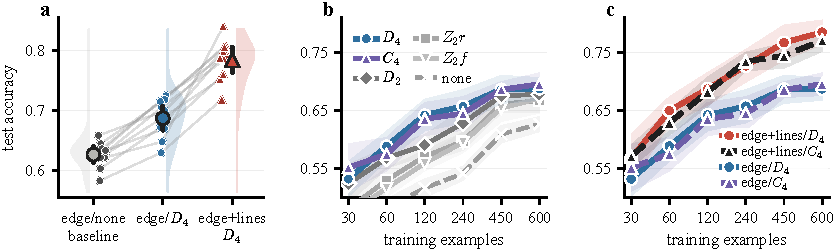
\includegraphics[width=.94\textwidth]{gfx/fig2_main_evidence}
\caption{\normalsize Main results. (a) Full $D_4$ improves over no sharing. (b) $C_4$ closely follows $D_4$ across train sizes. (c) Edge+lines gives the largest gain while preserving equivariance. Error bars are 95\% confidence intervals over seeds.}
\label{fig:main}
\end{figure*}


\section{Results}
\label{sec:results}
\Cref{fig:main} shows the main empirical story. In panel (a), the unconstrained edge ansatz carries many more parameters yet generalizes worse than the $D_4$-equivariant edge model. At 600 training examples, edge/none reaches about $0.63$ test accuracy while edge/$D_4$ reaches about $0.69$ with a smaller train-test gap. This reproduces the central lesson of Meyer et al.: the correct board symmetry removes irrelevant functions from the hypothesis class rather than simply shrinking the model.

Panel (b) makes the picture less binary. Full $D_4$ is the conservative default, but $C_4$ tracks it closely across the data grid: it is slightly ahead at 30 examples, and from 120 through 600 examples the two stay essentially together while weaker or unconstrained sharing lags. We read this cautiously. It does not establish that partial symmetry is generally better; it shows that symmetry strength is a tunable bias, with rotation-only equivariance preserving most of the benefit while relaxing reflection constraints. The random-sharing control in \cref{fig:controls}(a) is the guardrail: it fixes parameter count but scrambles the group-orbit structure, and performs substantially worse than orbit-based sharing at every subgroup. The useful prior is the board geometry, not just the smaller circuit.

The strongest effect, in \cref{fig:main}(c), comes from enriching the symmetry rather than weakening it. The original edge/$D_4$ model sits near $0.69$; adding both winning-line channels to the same equivariant circuit lifts the best $D_4$ model to roughly $0.80$, with the $C_4$ variant close behind. This is the central result: the gain comes not from abandoning symmetry, but from giving the equivariant ansatz direct access to the motifs that decide the label.

\Cref{fig:controls} rules out two simpler explanations. The gain is not arbitrary parameter reduction, since matched-size random sharing falls short of orbit sharing in panel (a). It is not simply more parameters either: edge+lines/$D_4$ has 90 parameters, more than edge/$D_4$ at 54 but far below the 204 of the unshared baseline. Panel (c) makes the point geometric: accuracy does not follow parameter count, and edge+lines models occupy a higher band at modest size. The ablation in panel (b) confirms the composition: line-only circuits help, but the strongest model combines local edge structure with both winning-line channels.

\begin{figure*}[t]
\centering
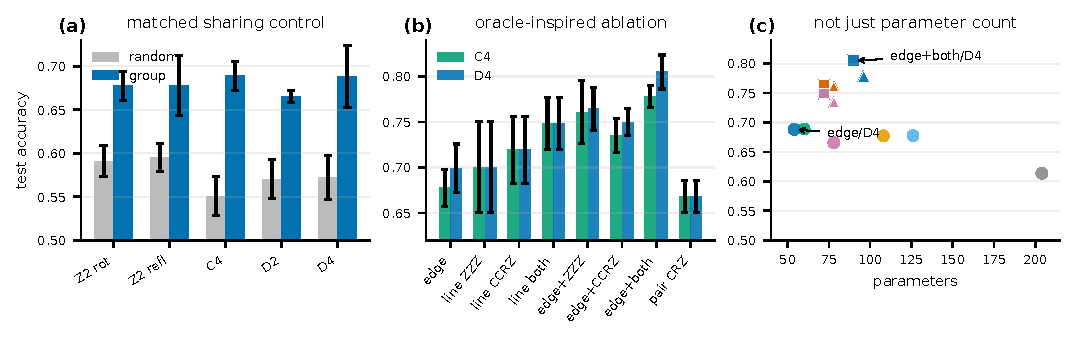
\includegraphics[width=.94\textwidth]{gfx/fig3_controls}
\caption{\normalsize Controls and ablations. (a) Parameter-matched random sharing underperforms group-orbit sharing. (b) Ablations are anchored by the labelled original edge/$D_4$ ansatz; the strongest model combines edge interactions with both line channels. (c) Accuracy is not explained by parameter count alone.}
\label{fig:controls}
\end{figure*}


\section{Discussion and Outlook}
\label{sec:discussion}
Our results support an architectural view of equivariance in variational quantum learning. Meyer et al. showed that incorporating task symmetry into a VQLM can improve generalization. We take this as a starting point and ask what remains to be designed once that symmetry has been imposed. The answer is that equivariance is not a complete ansatz specification: it constrains parameter sharing and responses to symmetry-related inputs, but not which trainable interactions the circuit should contain.

The subgroup experiments do not show that rotation-only equivariance is generally preferable to full board equivariance. They show that symmetry strength is a meaningful modeling choice. In this benchmark, weaker symmetry keeps most of the benefit of the fully symmetric model while giving the circuit slightly more freedom. Subgroup comparisons can therefore diagnose overconstraint when a fully equivariant circuit underperforms for a given data regime, circuit family, or optimizer.

The stronger empirical effect comes from changing the interactions inside the equivariant ansatz. The original edge circuit couples neighboring fields and must represent winning triples indirectly. The line interactions act directly on the three-cell structures that determine the label, while still sharing parameters across symmetry-related instances. This gives the largest improvement in our experiments. The matched random-sharing control rules out parameter reduction as the explanation: what matters is that trainable degrees of freedom are placed according to the task geometry.

This suggests a practical design principle. Once a task symmetry has been identified, one should ask not only whether the circuit respects it, but whether the equivariant gates expose the structures through which the label is determined. Equivariance is a starting point for ansatz design rather than its end point: it defines a constrained design space in which the choice of interactions can still be decisive.

Tic-Tac-Toe is small, enumerable, and exactly solvable by a deterministic rule oracle, so its value is as a controlled setting for isolating symmetry-aware architectural choices. The supported claim is narrow: task-aligned equivariant interactions can improve generalization while preserving the imposed symmetry. For larger problems, the transferable recipe is to identify task-relevant motifs and encode them as trainable interactions shared over the corresponding symmetry orbits.

A natural next step is to compare enriched equivariant ansatze with soft symmetry approaches, where controlled symmetry-breaking terms interpolate between hard equivariance and a free ansatz. Such comparisons should include not only the original symmetric circuit, but also equivariant circuits whose interactions have been designed to match the task. The broader lesson is that symmetry-aware quantum circuit design should use symmetry to organize the trainable interactions through which the model learns.


\section*{Appendix}
The code and experiment artifacts are in the project repository \url{https://github.com/eybmits/qc_symmetry}. All numerical claims in this draft are computed from checked CSV files in \texttt{results/csv/}. The exact sources are the reproduction file \path{results_reproduction.csv}, the subgroup file \path{results_partial_data_sweep_full_L3p2.csv}, the random-sharing file \path{results_random_sharing_control_full_L3p2_train450.csv}, and the oracle-gate file \path{results_oracle_inspired_robust_C4D4_L3p2_train450_600_750.csv}. Figures are regenerated by running \texttt{python paper/make\_figures.py}. The simulations use PennyLane~\cite{bergholm2018pennylane}, PyTorch~\cite{paszke2019pytorch}, NumPy, Pandas, and Matplotlib. Unless otherwise stated, models use $L=3$, $p=2$, batch size 15, 100 epochs, 30 minibatch steps per epoch, Adam~\cite{kingma2015adam} with learning rate $0.01$, and five seeds. The present draft is therefore a finite-seed simulation study; final submission should rerun the headline comparisons with 10--20 seeds.

The repository also contains experiment families that are not used as headline figures. The depth sweep tests whether the subgroup ordering changes with effective circuit depth $L p$; the compression sweep ties parameters more aggressively than $D_4$ to check whether still fewer parameters are sufficient; and the approximate-symmetry runs deliberately corrupt labels on a fraction of $D_4$ orbits. These runs are useful for paper development, but the current evidence is less central than the three claims reported here: reproduction, structured sharing, and winning-line architecture.

Several sanity checks are implemented directly in the codebase. The data generator enumerates legal reachable Tic-Tac-Toe states and verifies that labels are invariant under all eight $D_4$ transformations. The group module constructs transformations from board coordinates rather than hand-written permutations. The model checks compare trainable parameter counts with the orbit structure, and equivariance checks verify that subgroup-equivariant models give identical predictions on transformed boards up to numerical tolerance. The deterministic rule oracle is included only as a sanity reference: it confirms that the task is rule-solvable and that imperfect variational accuracy is a property of the ansatz and optimization, not of ambiguous labels.

The most important remaining limitation is statistical. Five seeds are enough to identify the architecture signal and to draft the paper, but they are not enough for a final robustness claim. The final version should rerun the reproduction and oracle-inspired comparisons with more seeds, report bootstrap intervals or nonparametric paired tests, and include finite-shot simulations if the work is framed toward hardware. The current claim is intentionally narrower: within exact-state simulation, task-aligned equivariant gates substantially improve a Meyer-style symmetric VQLM on a controlled benchmark.


\section*{Acknowledgment}
The authors thank Jonas Stein\orcid{0000-0001-5727-9151} for valuable discussions and feedback.

\bibliographystyle{IEEEtran}
\bibliography{references}

\end{document}
